\documentclass{bmvc2k}

%% Enter your paper number here for the review copy
% \bmvcreviewcopy{??}

% \usepackage[brazilian]{babel}
\usepackage[utf8]{inputenc}

\title{Image segmentation based\\ on color similarity}

% Enter the paper's authors in order
% \addauthor{Name}{email/homepage}{INSTITUTION_CODE}
\addauthor{Bruno Osorio}{osorio.bruno@hotmail.com.br}{1}

% Enter the institutions
% \addinstitution{Name\\Address}
\addinstitution{
  Department of Computer Science\\
  Universidade de Bras\'{\i}lia\\
  Campus Darcy Ribeiro, Asa Norte\\
  Bras\'{\i}lia-DF, CEP 70910-900, Brazil,  
}

\runninghead{Bruno, Osorio}{Computer Vision Assignment -- \today}

% Any macro definitions you would like to include
% These are not defined in the style file, because they don't begin
% with \bmva, so they might conflict with the user's own macros.
% The \bmvaOneDot macro adds a full stop unless there is one in the
% text already.
\def\eg{\emph{e.g}\bmvaOneDot}
\def\Eg{\emph{E.g}\bmvaOneDot}
\def\etal{\emph{et al}\bmvaOneDot}

%-------------------------------------------------------------------------
% Document starts here
\begin{document}

\maketitle

\begin{abstract}
This document covers the topic of image segmentation based on a simple technique of pixels selection. A comparison between a digital image and a reference color value is made for each pixel and only the pixels that satisfy a condition are selected to compose the segmented image. The comparison made is the Euclidean distance between the compared pixels and the condition to be met is a threshold rule.
\end{abstract}

%-------------------------------------------------------------------------
\section{Introduction}
\label{sec:intro}

The digital representation of a picture is a collection of \textit{pixels}~\cite{wiki-pixel}, i.e. Picture Elements, the smallest point in a digital image that holds the color information on a certain position in the image. Digital images are usually stored as a matrix of pixels with two dimensions due to the fact that the projection of a three-dimensional environment from a point of view results in a 2-D plane. One possible way to represent color in an image, is to store in each pixel the information of how red, green and blue the point represented by the pixel is. By emitting overlapping light rays with these three base color components in different intensities, any color within the visible spectrum can be displayed.

In computer vision, image segmentation~\cite{wiki-image-segmentation} is the name given to the process of extracting entities from an image, e.g., detecting a tree. Assuming that one entity has a single coloration, it's possible to extract this information by comparing other pixels in the image that have a similar color. Color similarity can be measured in many different ways, based on visual similarity, brightness etc.

The objective is to successfully separate an entity by comparing coloration in an image and generate an output image that highlights only the pixels that were extracted.

%-------------------------------------------------------------------------
\section{Methodology}
\label{sec:method}

The method used to measure the similarity between two pixels to exemplify the application of image segmentation based on color is the Euclidean distance~\cite{wiki-euclidean-distance}. Euclidean distance is the shortest distance between two points, i.e., the length of a straight line that connects two points. Euclidean distance between two points in a three dimensional space can be calculated by taking the square root of the sum of the squared differences between each coordinate, as shown in the following formula:

\[ d(p, q) = \sqrt{(p_1 - q_1)^2 + (p_2 - q_2)^2 + (p_3 - q_3)^2} \]

Two pixels are considered similar if the distance value between them is lower than a predetermined maximum value, called threshold. The threshold chosen to demonstrate the results of this technique was \textbf{13} (thirteen) as the color values intensities are all within the range \([0, 255] \). The color values of the components of each pixel can be viewed as three coordinates.

%-------------------------------------------------------------------------
\section{Results}
\label{sec:results}

Figure~\ref{fig:results_1} shows an example of an image with solid colors and high contrast alongside the result of a multiple segmentation processes based on different color values references.

\begin{figure}[!htb]
\begin{center}
\begin{tabular}{c c c c}
\fbox{
\includegraphics[width=0.18\linewidth]{Figs/rgb_blend.png}}&
\fbox{
\includegraphics[width=0.18\linewidth]{Figs/result-rgb-blend-black.png}}&
\fbox{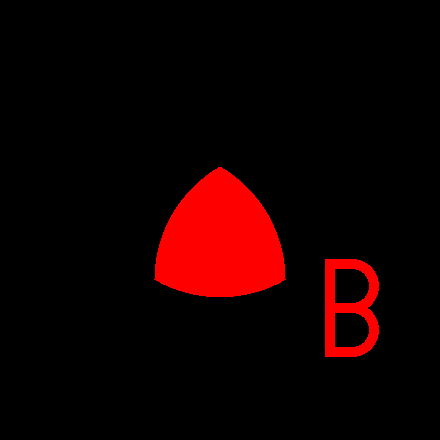
\includegraphics[width=0.18\linewidth]{Figs/result-rgb-blend-white.png}}&
\fbox{
\includegraphics[width=0.18\linewidth]{Figs/result-rgb-blend-green.png}}\\
(a)&(b)&(c)&(d)
\end{tabular}
\caption{(a) shows the original image used to demonstrate the segmentation; (b) shows the segmented pixels (painted red) when comparing the original image with the color \textit{black}; (c) shows the segmented pixels when comparing with \textit{white}; (d) shows the segmented pixels when comparing with \textit{green}.}
\label{fig:results_1}
\end{center}
\end{figure}

Figure~\ref{fig:results_2} shows an example of an image with huge variation of color values due to shading alongside the result of a segmentation process based on a skin color value reference.

\begin{figure}[!htb]
\begin{center}
\begin{tabular}{cc}
\fbox{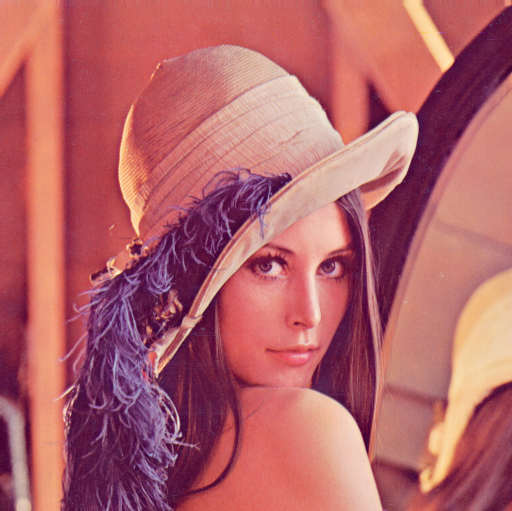
\includegraphics[width=0.32\linewidth]{Figs/lena-color.png}}&
\fbox{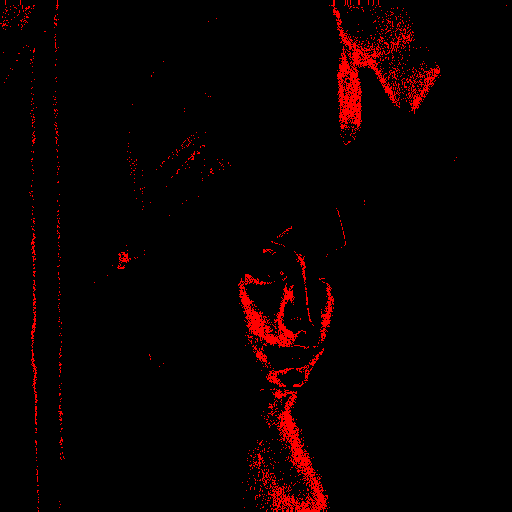
\includegraphics[width=0.32\linewidth]{Figs/result-lena-color.png}}\\
(a)&(b)
\end{tabular}
\caption{(a) shows the original image used to demonstrate the segmentation; (b) shows the segmented pixels (painted red) when comparing the original image with a skin color.}
\label{fig:results_2}
\end{center}
\end{figure}

%-------------------------------------------------------------------------
\section{Conclusion}
\label{sec:conclusion}

The presented technique is very simple and quick to implement and provides good results when dealing with images that are mainly composed of solid colors and entities that have almost no variation in its coloring. On the other hand, when applying this method to images that have many color shades and entities with complex color composition (like real life photographs), the technique is highly ineffective, since different pixels that belong to an entity will have a high Euclidean distance.

Another downside to this technique is that different entities with similar colors will be grouped together as the same entity. This can be observed in figure~\ref{fig:results_2} (b), as some parts of the background of the image have been selected despite the fact that those pixels do not belong to the person's skin. A possible solution to this problem could be enforcing a spatial relation between the selected pixels, in a way that similar pixels that are distant to a pixel, that is known to be part of the entity, will be less prone to be selected.

Although only one single value for threshold was analyzed in the examples, it's possible to alter this value and segment entities in a more restrictive way (lower threshold, less pixels selected) or in a more sensitive way (higher threshold, more pixels selected). As can be seen in figure~\ref{fig:results_2} (b), a relatively low value for the threshold resulted in only a few parts of the skin tone to be selected. Increasing the threshold could actually segment the person in the image more faithfully.

\bibliography{refs}
\end{document}
